\subsection{RLC en paralelo} \label{sec:RLC paralelo}
En esta sección, se estudió el comportamiento de un circuito RLC paralelo. Para esto, se montó el sistema de la figura \ref{fig:RLC-PARALELO}, con un resistor y un inductor conectados en serie entre sí y estos, a su vez, conectados a un capacitor en paralelo.
\begin{figure} [H]
    \centering
    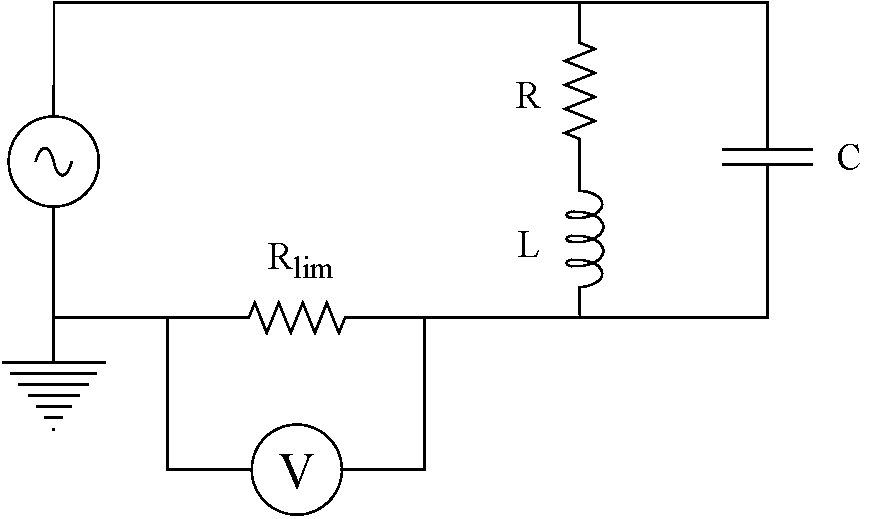
\includegraphics[width = 0.6\linewidth]{Esquemas/RLC-PARALELO.drawio.pdf}
    \caption{Esquema del circuito RLC paralelo formado por una fuente de tensión alterna $E=V_0\sen \omega t$, dos resistores, uno de resistencia $R_{lim}$ y el otro de resistencia $R$, un inductor de inductancia $L$ y un capacitor de capacitancia $C$. La resistencia $R_{lim}$ funciona como resistencia limitante, y se le conectó un voltímetro en paralelo para medir la caída de potencial sobre ella.}
    \label{fig:RLC-PARALELO}
\end{figure}
\paragraph{}
Este sistema posee una antirresonancia en la frecuencia $\omega_{0||}$ \eqref{eq:omega0 paralelo}, y con el ancho de su campana se puede definir el factor de calidad del sistema. El factor de merito \eqref{eq:Q RLC} depende de los valores de $R$, $L$ y $C$, por lo que modificando el valor de $R$, se modifica este factor.
\paragraph{}
La expresión de la tensión para este circuito es \eqref{eq:voltaje paralelo weak}
\begin{equation}\label{eq:voltaje paralelo weak}
    V_{ef}(\omega) = \frac{R_{lim}V_0}{|R_{lim} + Z_{||}|}.
\end{equation}
Reemplazando la expresión de la impedancia \eqref{eq:imp paralelo} en \eqref{eq:voltaje paralelo weak}, se puede obtener para la tensión la expresión \eqref{eq:voltaje paralelo}
\begin{equation}\label{eq:voltaje paralelo}
    V_{ef}(\omega) = \frac{A}{\sqrt{\big(
    B + \frac{(\frac{\omega}{\omega_0})^2}{\frac{1}{Q^2}+(\frac{\omega}{\omega_0} - \frac{\omega_0}{\omega})^2}
    \big)^2 + \frac{1}{Q^2}\big(
    \frac{Q^2(\frac{\omega}{\omega_0} - \frac{\omega_0}{\omega}) +  \frac{\omega_0}{\omega}}{\frac{1}{Q^2}+(\frac{\omega}{\omega_0} - \frac{\omega_0}{\omega})^2}\big)^2}},
\end{equation}
donde $A = V_0 R_{lim}/R$ y $B = R_{lim}/R$. Para calcular la diferencia de fase, se reemplazan los parametros del problema en \eqref{eq:fase weak} y se obtiene la expresión \eqref{eq:fase paralelo}
\begin{equation}\label{eq:fase paralelo}
    \Delta\phi(\omega) = \arctan\left(\frac{1}{Q}\frac{
    Q^2(\frac{\omega}{\omega_0} - \frac{\omega_0}{\omega}) +  \frac{\omega_0}{\omega}
    }{
    B(\frac{1}{Q^2} + (\frac{\omega}{\omega_0} - \frac{\omega_0}{\omega})^2) + (\frac{\omega}{\omega_0})^2
    }\right).
\end{equation}
\paragraph{}
Se realizó un barrido de frecuencias y se registró la caída de tensión en $R_{lim}$ y el defasaje para dos valores de $R$, con $R_1\ll R_2$. El valor de $R$ modifica significativamente el ancho de la campana y, por lo tanto, el factor de mérito. Se realizó el mismo procedimiento de recolección de datos que en la sección \ref{sec:RLC serie}. Se realizó un ajuste con la ecuación \eqref{eq:voltaje paralelo} y, con los coeficientes obtenidos, se calculó la potencia disipada en $R_{lim}$. En la figura \ref{fig:paralelo potencia1} se encuentran el gráfico de la tensión en función de la frecuencia y la potencia disipada por la resistencia $R_{lim}$ en función de $\omega/\omega_{0||}$ para el primer valor de resistencia. 
\begin{figure} [H]
    \centering
    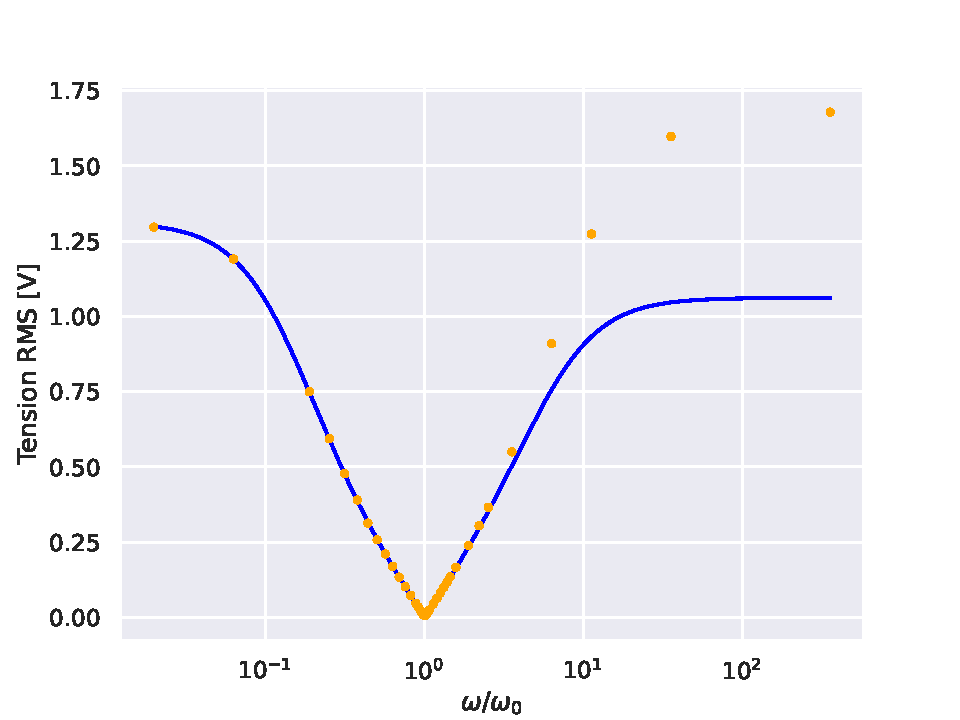
\includegraphics[scale=0.5]{figuras/RLC-PARALELO-1/tension.pdf}
    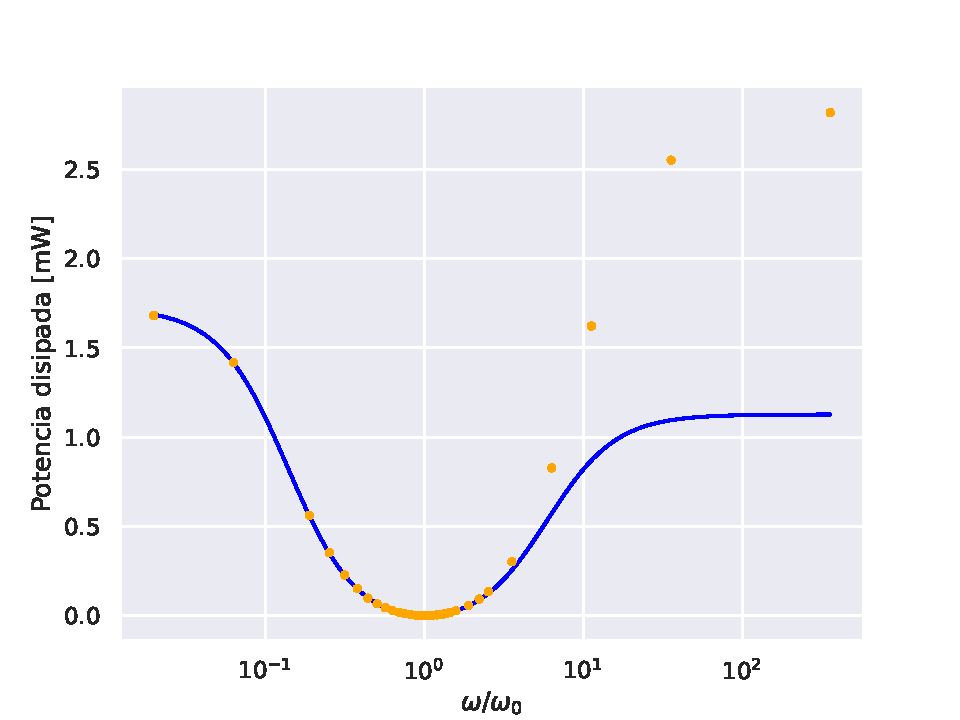
\includegraphics[scale=0.45]{figuras/RLC-PARALELO-1/potencia.pdf}
    \caption{Gráfico de la tensión del circuito con $R_1$ en función de la frecuencia, con los datos medidos en naranja y el ajuste en azul (izquierda). Gráfico de la potencia  en función de utilizando los coeficientes obtenidos del ajuste. En naranja, se aplicó la ecuación \eqref{eq:potencia generica} a los datos. En azul, se aplicó la ecuación \eqref{eq:potencia generica} a la función obtenida del ajuste (derecha). Los residuos  presentan una distribución aparentemente aleatoria y $R^2=0.91$, por lo que el ajuste es confiable.}
    \label{fig:paralelo potencia1}
\end{figure}
\paragraph{}
Debido a las limitaciones del modelo, en el ajuste se excluyeron valores de frecuencia del orden de $10^4\,$Hz. El valor de la frecuencia de resonancia  encontrado (utilizando la expresión  \eqref{eq:frec angular a frec}) fue de $f_{0||}=(1589.45\pm 0.02)\;$Hz. El factor de merito calculado fue de $Q_1=31.43\pm 0.03$. Como se puede observar en el gráfico a la derecha de la figura \ref{fig:paralelo potencia1}, el modelo se ajusta muy bien hasta valores de $\omega/\omega_{0||}$ del orden de $10^{1}$, pero falla cuando esta relación es mayor.
\paragraph{}
Se realizaron los diagramas de Bode del defasaje y la atenuación para esta resistencia,  y estos se muestran en la figura \ref{fig:paralelo bode1}. Para obtener la diferencia de fase, se ajustó mediante la ecuación \eqref{eq:fase paralelo}, utilizando los coeficientes obtenidos previamente.
\begin{figure} [H]
    \centering
    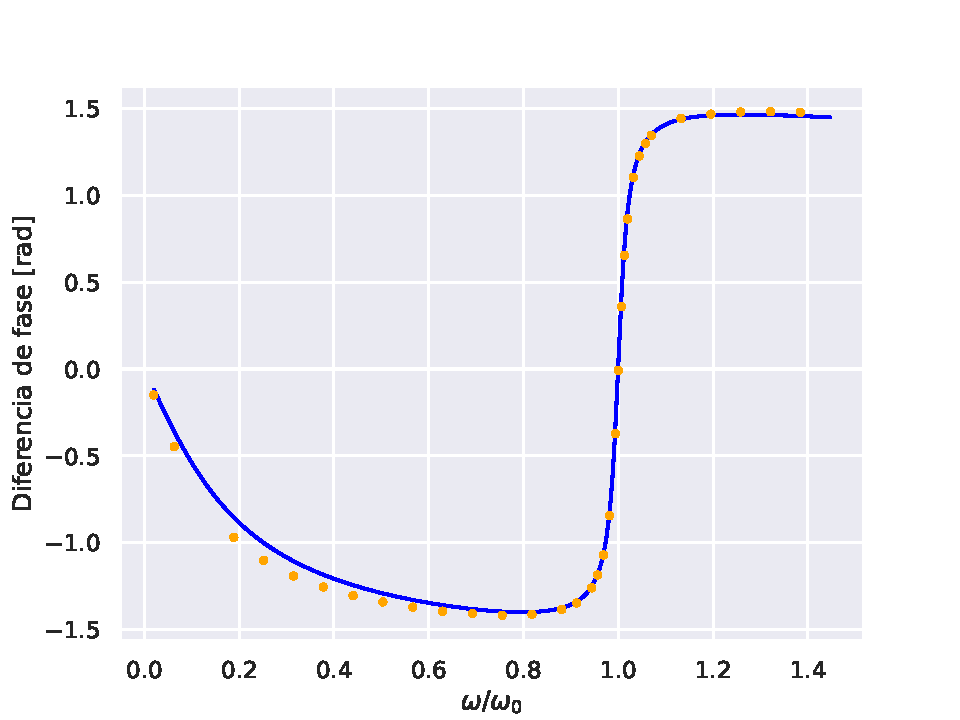
\includegraphics[scale=0.5]{figuras/RLC-PARALELO-1/fase.pdf}
    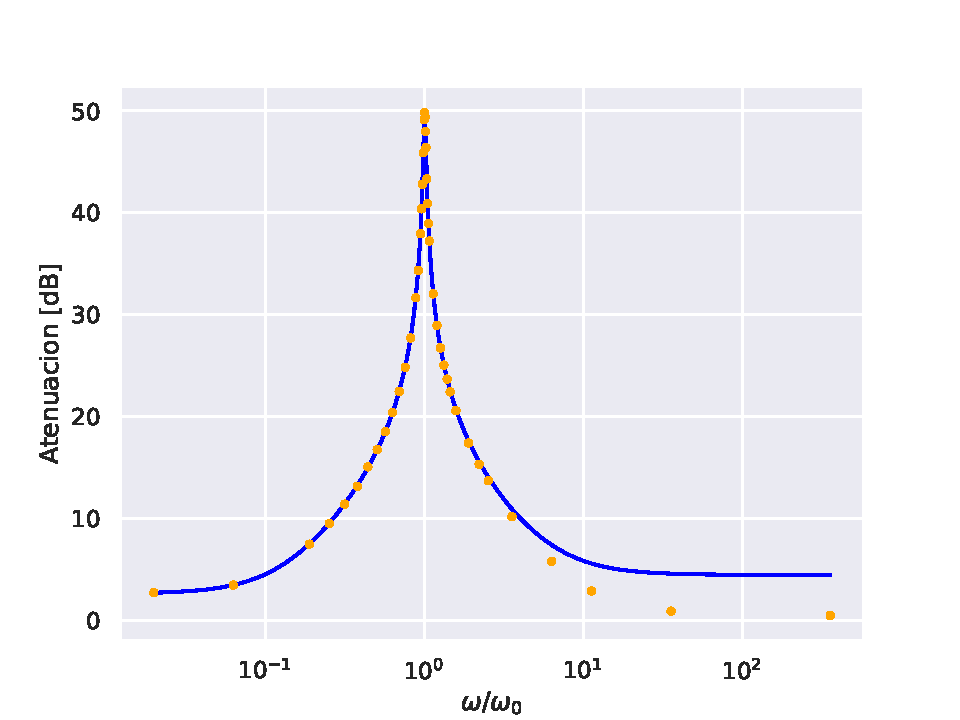
\includegraphics[scale=0.5]{figuras/RLC-PARALELO-1/atenuacion.pdf}
    \caption{Gráfico de la diferencia de fase. En naranja, la diferencia de fase medida y en azul, el ajuste (izquierda). Gráfico de la atenuación reemplazando los datos (naranja) y el ajuste de la tensión (azul) en la ecuación \eqref{eq:atenuacion} (derecha).}
    \label{fig:paralelo bode1}
\end{figure}
\paragraph{}
 Como se puede observar en la figura \ref{fig:paralelo bode1}, el modelo se ajusta muy bien alrededor de $\omega/\omega_0=1$, pero falla a frecuencias menores a $\omega_0$. Esto se puede deber a que el modelo no representa del todo el circuito real, es decir, que hay factores que el modelo no tiene en cuenta.
\paragraph{}
Se recolectaron los datos para el segundo valor de $R$, se realizó el ajuste de los datos con la ecuación \eqref{eq:voltaje paralelo} y se calculó la potencia. En la figura \ref{fig:paralelo potencia2} se muestran ambos gráficos.
\begin{figure} [H]
    \centering
    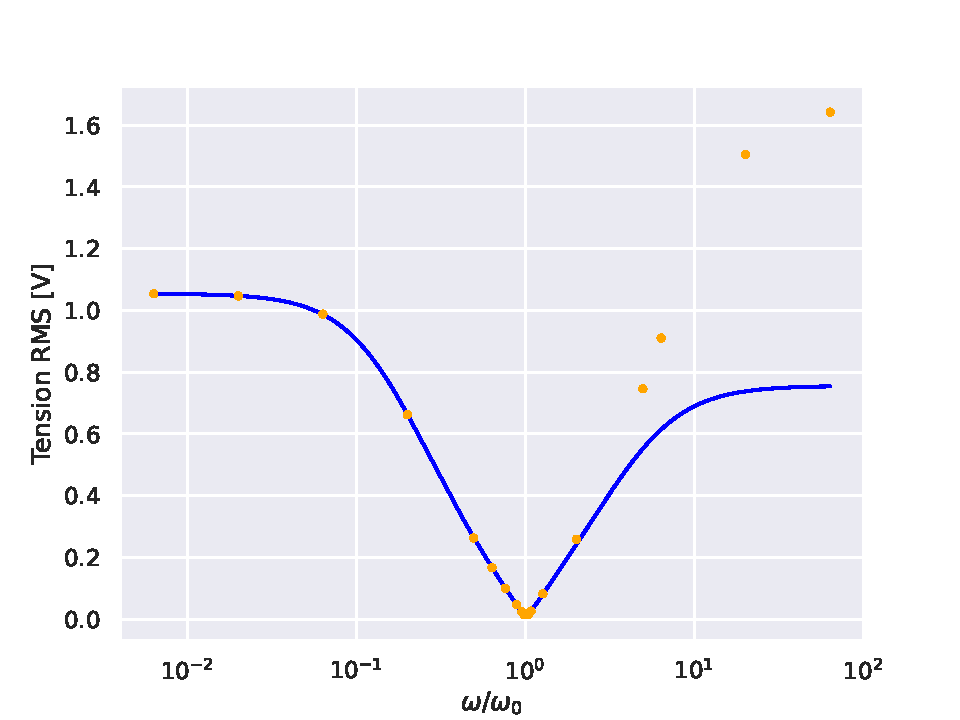
\includegraphics[scale=0.5]{figuras/RLC-PARALELO-2/tension_bode.pdf}
    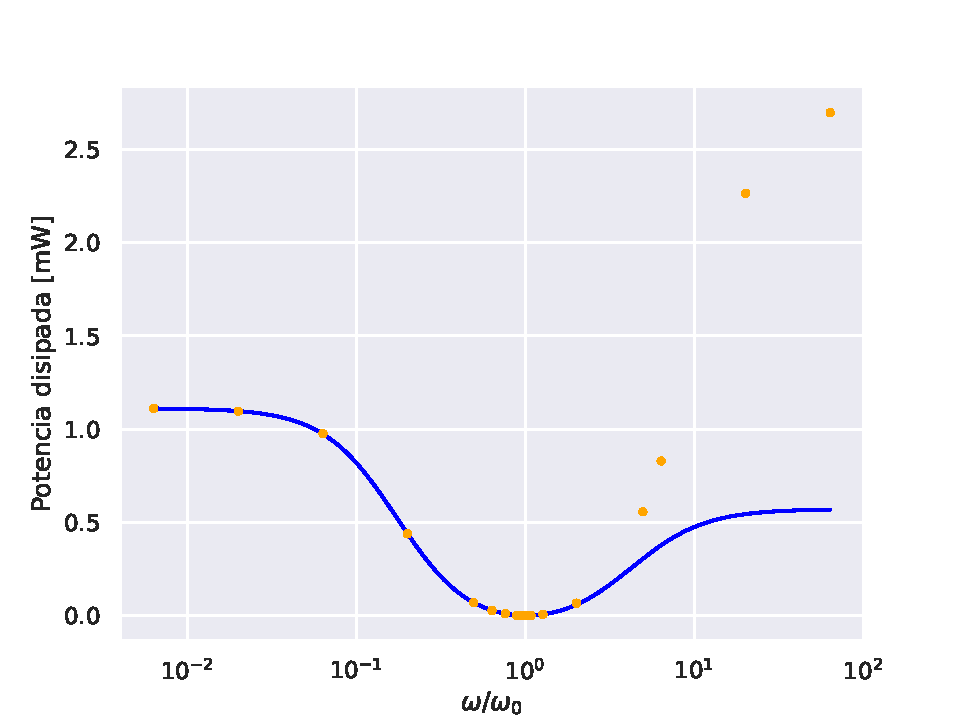
\includegraphics[scale=0.5]{figuras/RLC-PARALELO-2/potencia.pdf}
    \caption{Gráfico de la tensión del circuito con el segundo valor de $R$ en función de la frecuencia, con los datos medidos en naranja y el ajuste en azul (izquierda). Gráfico de la potencia  en función de utilizando los coeficientes obtenidos del ajuste. En naranja, se aplicó la ecuación \eqref{eq:potencia generica} a los datos. En azul, se aplicó la ecuación \eqref{eq:potencia generica} a la función obtenida del ajuste (derecha). Los residuos  presentan una distribución aparentemente aleatoria y $R^2= 0.72$, por lo que el ajuste es confiable.}
    \label{fig:paralelo potencia2}
\end{figure}
\paragraph{}
Al igual que en la figura \ref{fig:paralelo potencia1}, el modelo usado para el ajuste de la tensión falla cuando $\omega/\omega_0$ es mucho mayor a $1$. Esto se debe a que el modelo no es el correcto para describir el circuito a altas frecuencias, está incompleto. Sin embargo, se puede calcular una frecuencia de resonancia utilizando este de este sistema, ya que el modelo sí funciona alrededor de dicha frecuencia, y se obtuvo $f_{0||}=(1584.16\pm 0.05)\;$Hz. El factor de mérito de este circuito es $Q_2=15.24\pm0.02$.
\paragraph{}
Se realizaron los diagramas de Bode del defasaje y la atenuación para la segunda resistencia, los cuales se observan en la figura \ref{fig:paralelo bode2}. Para obtener la diferencia de fase, se ajustó mediante la ecuación \eqref{eq:fase paralelo}, utilizando los coeficientes obtenidos previamente.
\begin{figure} [H]
    \centering
    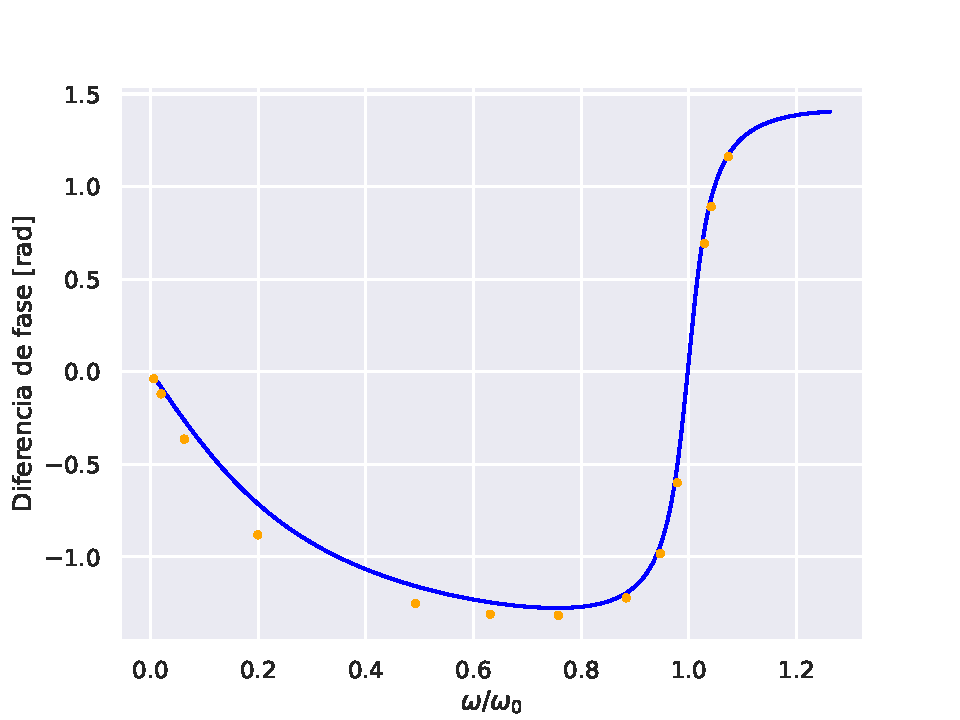
\includegraphics[scale=0.5]{figuras/RLC-PARALELO-2/fase.pdf}
    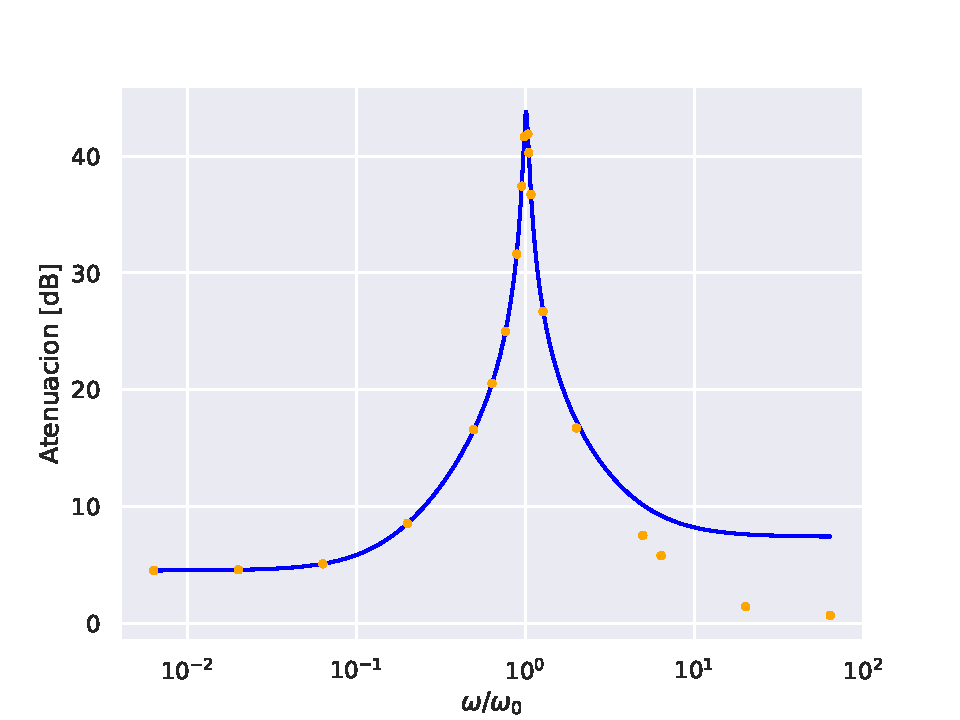
\includegraphics[scale=0.5]{figuras/RLC-PARALELO-2/atenuacion.pdf}
    \caption{Gráfico de la diferencia de fase; en naranja, la diferencia de fase medida y en azul, el ajuste (izquierda). Gráfico de la atenuación reemplazando los datos (naranja) y el ajuste de la tensión (azul) en la ecuación \eqref{eq:atenuacion} (derecha).}
    \label{fig:paralelo bode2}
\end{figure}
Al igual que en la figura \ref{fig:paralelo bode1}, el modelo utilizado para el ajuste de la diferencia de fase no es el correcto para las frecuencias menores a $\omega_0$. En el gráfico de la atenuación, el modelo falla en frecuencias mucho mayores a $\omega_0$.
\paragraph{}
Los factores de mérito \eqref{eq:Q RLC} cumplen la relación $Q_1\gg Q_2$. Esto es razonable, ya que $R_1 > R_2$.